\documentclass[5p,twocolumn]{elsarticle}
\usepackage{amsmath,amssymb,mathtools,amsthm}
\usepackage{graphicx,booktabs,multirow,microtype,xcolor}
\usepackage{lmodern}
\usepackage{algorithm,algpseudocode}
\usepackage{xurl}
\usepackage{placeins}
\usepackage{balance}
\usepackage[colorlinks=true,allcolors=black]{hyperref}
\newtheorem{proposition}{Proposition}
\newcommand{\StableKG}{StableKG}
\graphicspath{{../../figures/neurocomputing/}}
\journal{Neurocomputing}
\renewcommand{\topfraction}{0.95}
\renewcommand{\dbltopfraction}{0.95}
\renewcommand{\dblfloatpagefraction}{0.85}
\renewcommand{\floatpagefraction}{0.85}
\renewcommand{\textfraction}{0.05}
\setlength{\emergencystretch}{1.5em}
\begin{document}
\hypersetup{allcolors=black}
\hypersetup{pdftitle={Exact stability certificates for neural temporal knowledge graph completion},pdfauthor={Yanbo Bian}}
\raggedbottom
\begin{frontmatter}
\title{Exact stability certificates for neural temporal knowledge graph completion}
\author[inst]{Yanbo Bian\corref{cor}}
\ead{24722081@bjtu.edu.cn}
\cortext[cor]{Corresponding author.}
\affiliation[inst]{organization={Weihai International College, Beijing Jiaotong University},city={Weihai},postcode={264401},country={China}}
\begin{abstract}
Neural knowledge systems need to manage the evidence behind an answer when that evidence can be revised. Prediction confidence alone does not specify whether an answer survives the withdrawal of a coherent period of observations. We introduce StableKG, an editable temporal-memory interface with exact stability certificates for neural temporal knowledge graph completion. The interface combines a frozen neural distribution with a memory distribution that is renormalized after deletion. Multiplying a post-deletion pairwise margin by its retained-mass fraction reduces certification to an additive optimization, yielding an exact adversary and a constructive deletion witness. A sparse competitor theorem preserves the full-vocabulary guarantee, and a reverse index enables local maintenance. Experiments with two backbones and three training seeds on ICEWS14 and ICEWS05-15 show that certificate surplus improves deletion-flip discrimination over the original score margin by 0.064--0.584 AUROC across 16 perturbation comparisons. At 40\% coverage, certified selection eliminates worst-window flips for the compact backbone and reduces the joint rate of incorrect or edit-sensitive answers by 11.07 and 4.05 percentage points on the two datasets. Across 240 edit transactions, including a 2.3-million-event GDELT history, local maintenance reduces query-state refreshes by 95.41\%. These results establish an explicit, computable tolerance to evidence withdrawal as a complementary capability of neural graph prediction.

\end{abstract}
\begin{keyword}
Temporal knowledge graph \sep Certified robustness \sep Selective prediction \sep Knowledge editing \sep Incremental inference
\end{keyword}
\end{frontmatter}
\section{Introduction}
Evidence in temporal knowledge graphs can change after an answer has been issued. Events from the same observation period may be withdrawn together, leaving a system to decide which answers remain usable. A high prediction score does not reveal whether an answer depends on one such period or survives the removal of several. An explicit tolerance to evidence withdrawal would make that decision inspectable and allow the system to revisit only the affected answers.

\begin{figure*}[!t]
\centering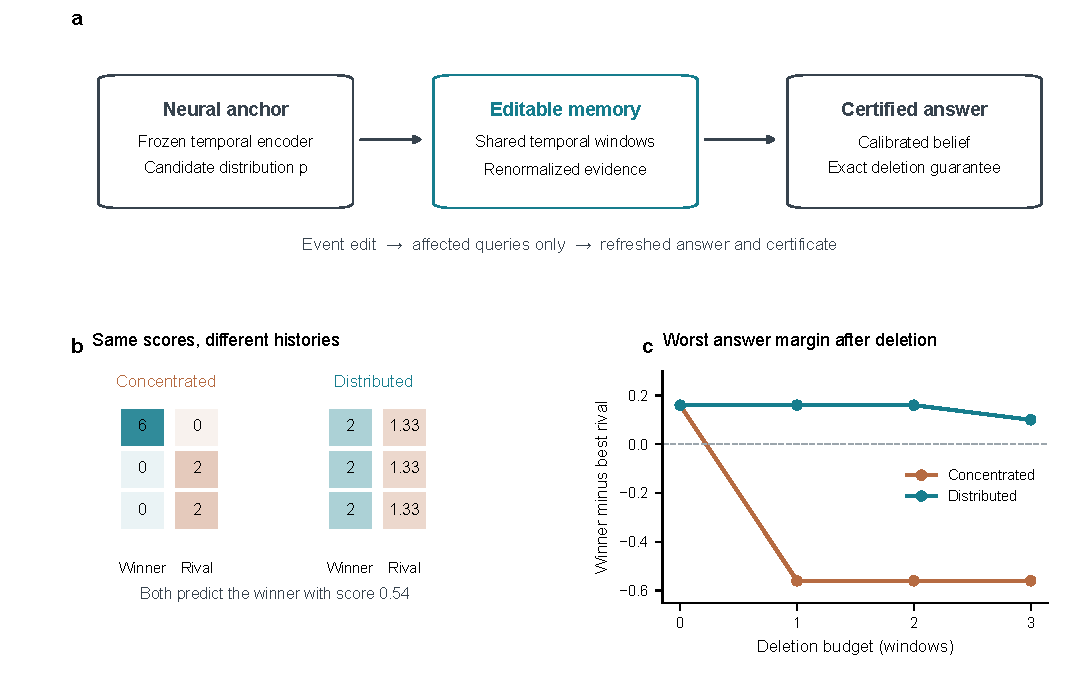
\includegraphics[width=\textwidth]{fig01_interface.pdf}
\caption{\textbf{Evidence organization creates a stability question beyond prediction scores.}
\textbf{a,} A frozen neural anchor and an editable temporal memory provide the distributions used for prediction, calibrated selection and exact deletion certification. Event edits refresh the affected registered queries.
\textbf{b,} A conceptual example with neural probabilities $(0.45,0.35,0.20)$ and evidence weight $0.6$. Both histories have total object masses $(6,4,0)$ and the same score vector $(0.54,0.38,0.08)$, but distribute their support differently across three windows. Distributed rival masses are exactly $4/3$ per window, rounded in the display.
\textbf{c,} Exhaustive deletion of at most the indicated number of windows yields different worst-case winner margins. These values illustrate the construction and are not empirical benchmark results. The schematic and plotting code were prepared with assistance from OpenAI Codex (OpenAI; desktop build 26.915.4065.0 recorded during final preparation).}
\label{fig:interface}
\end{figure*}


Temporal knowledge graph completion has developed increasingly expressive representations of event history. Recent methods model temporal granularity, cross-space interactions and frequency-dependent relations \citep{geng2025granularity,vu2025tcrosse,liu2025terdy}. History extraction, multiple temporal views and state embeddings supply complementary information for predicting missing facts \citep{dao2025hgct,chen2025dualview,ji2025stse}. Newer work extends these representations through Householder transformations, sparse fact aggregation and tensorized temporal relations \citep{xu2026householder,zhu2026splices,lee2026tirano}. These advances improve the predictive model. They also make it valuable to attach an explicit account of how an exposed answer responds to a change in its observable evidence.

Predictive confidence and resistance to evidence deletion address different questions. Calibration estimates how often a prediction is correct, while selective prediction uses a confidence score to determine which answers to expose. Recent uncertainty and rejection methods strengthen this statistical decision layer \citep{liu2025uncertkg,li2025vicinal,szabadvary2025reject,he2025conjunction}. Temporal conformal prediction additionally addresses dependence between graph observations \citep{wang2025nonexchangeable}. An evidence-deletion certificate instead concerns one fixed query: it states that every allowed deletion preserves the answer. Even two queries with the same score vector can have different certificates when their evidence is arranged differently across time (Fig.~\ref{fig:interface}). A useful decision layer should preserve this distinction while making both quantities available at inference time.

We introduce \StableKG{}, an editable evidence interface for neural temporal knowledge graph completion. A frozen neural predictor supplies an anchor distribution, and a temporal memory supplies a second distribution over candidate objects. The memory is renormalized after evidence is deleted. Although this normalization couples all object scores, the sign of each post-deletion winner--competitor margin reduces to an additive expression. Sorting its positive window contributions identifies an exact worst-case deletion without enumerating subsets. A further reduction checks only evidence-supported objects and one additional neural competitor, while a reverse index restricts maintenance to queries affected by an event edit.

The resulting system provides three concrete capabilities: an exact certificate for coherent temporal-window deletion, a selective policy that combines the certificate with calibrated correctness, and local maintenance of predictions and certificates. We evaluate the interface with two temporal neural backbones and three training seeds on ICEWS14 and ICEWS05-15, then examine maintenance on a 2.3-million-entry GDELT history. The experiments measure predictive performance, empirical selection error, intervention sensitivity and computational cost. Together, they connect a formal tolerance to evidence withdrawal with the prediction and maintenance behavior of neural knowledge systems.

\section{Related work}
\paragraph{Temporal representations and evidence selection.}
Current temporal reasoning models combine information at several time scales. Multi-granularity history graphs and hybrid history networks aggregate complementary views of the past \citep{zhu2025multigran,ye2026dualhistory}; semantic dual graphs and frequency-aware interactions enrich relation modeling \citep{zhang2026dstag,wang2026multidim}. Sparse-graph reasoning, global structural interaction and cyclic evolution address further aspects of incomplete histories \citep{peng2026icpe,wang2026globalinteraction,bi2026globallocal}. These developments motivate a modular interface that can be attached to different temporal predictors. Our experiments use the author implementation of TeRDy \citep{liu2025terdy} and a compact temporal factorization model, keeping each encoder fixed while its explicit memory is edited.

\paragraph{Interpretability and knowledge editing.}
Temporal rule validity, logical paths and semantic dependencies make parts of the reasoning process accessible to inspection \citep{pan2025validity,zhang2026logicalpaths,yu2026dependency}. Graph--text alignment and in-context contrastive learning connect structured history with additional representations \citep{wan2026tgcallm,li2026calendar}. IGETR combines temporal graph paths with language-model-guided editing to improve interpretable reasoning \citep{fan2026editing}. \StableKG{} considers a different operation: a specified family of deletions to the inference-time evidence channel, with a computable guarantee for the resulting answer. The edit acts on an explicit memory; the learned encoder remains the same throughout the transaction.

\paragraph{Selection and robustness guarantees.}
Recent selective-classification methods use conformal rejection, conjunction tests or additional pairwise queries to improve the decision to answer \citep{szabadvary2025reject,he2025conjunction,vardhan2026pairwise}. NCPNET develops conformal prediction for non-exchangeable temporal graphs \citep{wang2025nonexchangeable}. Robustness certification provides another type of guarantee: GraphProt uses a sampled subgraph ensemble against graph backdoors \citep{yang2025graphprot}, and AdaptDel studies variable-rate deletion smoothing for sequence classifiers \citep{huang2025adaptdel}. Our certificate is deterministic and exact for the defined neural--memory score and shared-window deletion family. Its tractability follows from the ratio-to-additive reduction and sparse competitor structure. The experiments therefore compare exact certification with a conservative analytical bound and random deletion probes, while comparing answer selection against confidence, margin, entropy, temperature scaling and ensemble controls. Recent work on sharpness and bias in graph completion further motivates reporting these distinct evaluation axes explicitly \citep{moon2026sharpness}.

\section{Method}
\subsection{Task and editable evidence interface}
A temporal fact is a quadruple $(s,r,o,t)$ containing a subject, relation, object and timestamp. For a query $q=(s,r,?,t_q)$, let $\mathcal A_q$ be the entity vocabulary excluding objects already observed in the training graph for exactly $(s,r,t_q)$. This exclusion is determined entirely by observed training facts. The candidate vocabulary remains fixed during an edit experiment.

A trained temporal encoder produces logits $z_\theta(q,o)$. The neural anchor is
\begin{equation}
p_q(o)=\frac{\exp\{z_\theta(q,o)/T\}}{\sum_{v\in\mathcal A_q}\exp\{z_\theta(q,v)/T\}},\qquad o\in\mathcal A_q,
\label{eq:anchor}
\end{equation}
where $T>0$ is selected on validation data. The editable memory contains training events $(s,r,o,t_e)$ with $t_e\le t_q$ and $o\in\mathcal A_q$. Each event receives weight $2^{-(t_q-t_e)/h}$, with half-life $h$. Events are grouped into shared windows $b=\lfloor t_e/\omega\rfloor$. Define
\begin{equation}
\begin{aligned}
e_{bo}&=\sum_{e:\,o_e=o,\,b_e=b}2^{-(t_q-t_e)/h},\\
E_o&=\sum_b e_{bo},\quad m_b=\sum_o e_{bo},\quad S=\sum_b m_b.
\end{aligned}
\label{eq:memory}
\end{equation}
Only nonempty windows are retained. The original prediction score is
\begin{equation}
g(o)=(1-\lambda)p_q(o)+\lambda E_o/S,\qquad 0\le\lambda<1.
\label{eq:fusion}
\end{equation}
When $S=0$, the score is $p_q(o)$. Thus the interface is a mixture of two distributions over the same admissible candidates. It can change a neural answer when temporal evidence supplies a stronger alternative, and it reduces to the neural predictor when no admissible history is available.

The published benchmark split is interpolative: the neural encoder learns from the full published training split. The temporal cutoff in Eq.~\eqref{eq:memory} governs the editable memory. Encoder parameters, query timestamps and the candidate vocabulary are fixed while that memory is edited.

\subsection{Exact certification under shared-window deletion}
Deleting a shared window removes its events for \emph{every} candidate. For a proper subset $D$ of the $B$ nonempty windows, the edited score is
\begin{equation}
g_D(o)=(1-\lambda)p_q(o)+\lambda\frac{E_o-\sum_{b\in D}e_{bo}}{S-\sum_{b\in D}m_b}.
\label{eq:edited}
\end{equation}
Deleting all evidence returns the neural anchor. Let $w=\arg\max_o g(o)$, with ties resolved by the smallest entity identifier. For each competitor $c\ne w$, define the original gap $G_c=g(w)-g(c)$ and signed window contribution
\begin{equation}
d_{bc}=\lambda\frac{e_{bw}-e_{bc}}{S}
 +(1-\lambda)\{p_q(w)-p_q(c)\}\frac{m_b}{S}.
\label{eq:delta}
\end{equation}
The first term measures the evidence advantage lost when a window is deleted. The second accounts for renormalization relative to the neural anchor. Both the winner's support and the competitor's support therefore enter the same intervention.

\begin{proposition}[Exact shared-window certificate]
For any proper deleted subset $D$,
\begin{equation}
\left(1-\sum_{b\in D}\frac{m_b}{S}\right)\{g_D(w)-g_D(c)\}
=G_c-\sum_{b\in D}d_{bc}.
\label{eq:reduction}
\end{equation}
Consequently, the largest loss of the signed gap numerator over proper subsets with $|D|\le k$ is the sum of the largest $\min(k,B-1)$ positive values of $d_{bc}$. Checking this sum for every competitor, together with the neural fallback when $k\ge B$, determines exactly whether every allowed deletion preserves $w$.
\label{prop:certificate}
\end{proposition}

Equation~\eqref{eq:reduction} follows by multiplying the score difference by the positive retained-mass fraction. A cardinality-bounded sum is maximized by choosing its largest positive terms. If its remaining numerator is negative, those windows provide a constructive deletion witness. A zero numerator is resolved by the fixed tie rule. The complete-deletion case is checked separately because its denominator is zero. These observations prove Proposition~\ref{prop:certificate}; Supplementary Information gives the full case analysis.

We call the minimum signed gap numerator across competitors the \emph{certificate surplus}. If complete deletion is allowed and changes the answer, the minimum also includes its negative neural fallback gap. Together with the tie rule, the surplus sign determines stability; its magnitude is not the unscaled post-edit margin. The certificate radius is the largest budget that retains the answer, capped at $B$. Empty memory is stable because there is no editable evidence, and its frequency is reported separately. For long histories, implementation uses suffix sums of the retained masses after sorting, preserving small old contributions when recent mass is removed.

\subsection{Sparse certification over the full vocabulary}
\begin{proposition}[Sparse competitor reduction]
Let $\mathcal C_q=\{o:E_o>0\}$ be the evidence support. It is sufficient to check competitors in $\mathcal C_q\setminus\{w\}$ and the highest-probability neural candidate outside $\mathcal C_q\cup\{w\}$.
\label{prop:sparse}
\end{proposition}
Every unsupported candidate has zero memory mass before and after deletion. Their score ordering is therefore their neural ordering for all allowed edits, including the complete-deletion fallback. The best unsupported candidate dominates every other unsupported competitor, proving Proposition~\ref{prop:sparse}.

After neural logits are available, finding the winner and unsupported representative takes $O(N)$ time for $N$ admissible candidates. With $C$ supported competitors and $B$ windows, sorting the signed contributions costs $O(CB\log B)$ and the window statistics occupy $O(CB)$ memory. This replaces subset enumeration and avoids sorting contributions for all $N$ candidates. Algorithm~\ref{alg:certificate} summarizes the procedure.

\begin{algorithm}[t]
\caption{Exact certification of a neural--memory prediction}
\label{alg:certificate}
\begin{algorithmic}[1]
\Require Frozen anchor $p_q$, nonempty window masses $e_{bo}$, weight $\lambda$, budget $k$
\State Form $g$ using Eq.~\eqref{eq:fusion}; select winner $w$
\State Identify supported competitors and the best unsupported candidate
\For{each retained competitor $c$}
  \State Compute $d_{bc}$ using Eq.~\eqref{eq:delta}
  \State Sort contributions; retain up to $\min(k,B-1)$ positive terms
  \State Compute retained winner, competitor and total masses by suffix sums
  \If{$c$ overtakes $w$, including the tie rule}
    \State \Return uncertified, with the corresponding deletion witness
  \EndIf
\EndFor
\If{$k\ge B$ and the neural fallback changes $w$}
  \State \Return uncertified, with the complete-deletion witness
\EndIf
\State \Return certified
\end{algorithmic}
\end{algorithm}

\subsection{Confidence and certified selection}
For each predicted answer, a ridge logistic model estimates its probability of belonging to the published known-answer set. Its inputs are fitted on validation data and then fixed. We compare score-only features, additional evidence descriptors, and additional certificate descriptors. The latter include the one- and two-window surpluses, their certificate indicators and the radius divided by the number of windows. A separate calibration control uses only the hybrid maximum score.

The deployed belief model is selected among these one-encoder calibrators by validation area under the risk--coverage curve (AURC). For a belief threshold $\tau$ and deletion budget $k$, acceptance is
\begin{equation}
\begin{aligned}
\mathrm{accept}(q)={}&\mathbf 1\{\widehat P(\mathrm{correct}\mid q)\ge\tau\}\\
&\times\mathbf 1\{q\text{ is certified for budget }k\}.
\end{aligned}
\label{eq:accept}
\end{equation}
The two factors have different roles: calibration estimates empirical correctness, and the certificate guarantees invariance within the specified edit family. Exact-coverage comparisons sort the same predictions and select the requested number of certified candidates. If too few candidates are certified, that operating point is reported as unavailable. Deployment results instead use thresholds fixed on the operating-validation subset and report their realized test coverage.

\subsection{Local maintenance after an event edit}
Each registered query caches its frozen anchor, admissible vocabulary and window statistics. A reverse index maps $(s,r)$ to registered query identifiers. An edit to $(s,r,o,t_e)$ affects only queries with that key, $t_q\ge t_e$, and $o\in\mathcal A_q$. Updating the corresponding window cell and total mass is sufficient to refresh the query's score, winner and certificate. Queries outside this set remain unchanged by Eqs.~\eqref{eq:memory}--\eqref{eq:edited}. This establishes exact local maintenance for the inference interface. The benchmark compares it with a full refresh that maintains the same indexed statistics and recomputes every registered query.

\section{Experimental design}
\subsection{Public data and prediction protocol}
We use ICEWS14 and ICEWS05-15 in the public TFLEX point-query distribution. Their training graphs contain 72,826 and 368,962 event entries and their vocabularies contain 7,128 and 10,488 entities, respectively. Each dataset supplies 5,000 validation queries and 5,000 test queries, selected at evenly spaced positions in the published source order without using labels. Every held-out target in these two panels is absent from the training facts at the query timestamp. The raw archives, immutable source revisions and SHA-256 hashes are recorded in the data manifest.

For filtered ranking, each designated held-out answer is ranked after removing the other known true answers for that query. Equal scores receive average ranks. We report mean reciprocal rank (MRR) and Hits@1/3/10, averaging over designated answers. For selective prediction, the system chooses one admissible object without accessing held-out labels. Validation labels and filtering use training and validation facts only; test facts do not enter checkpoint, fusion or selector decisions. Final test correctness uses the complete published known-answer set, so another known true answer is not counted as an error merely because it occurs in a different split. Training-observed answers remain excluded from selection. Thus selective answer-set accuracy and target-wise filtered Hits@1 describe related but different outcomes.

GDELT supplies a separate maintenance experiment with 2,308,165 training-event entries and 500 entities. Its prediction anchor is a fixed relation-frequency distribution estimated from training counts with unit pseudocounts. This experiment isolates cache scaling on a dense public history; neural completion results are reported on the two ICEWS datasets.

\subsection{Backbones, training and validation roles}
TeRDy uses the authors' model and regularizers at a pinned repository commit \citep{liu2025terdy}. The embedding ranks are 6,000 for ICEWS14 and 2,000 for ICEWS05-15. We train up to 36 and 24 epochs, respectively, with checkpoint evaluation every three and two epochs and patience of four validation checks. Optimization uses the published Adagrad learning rates and regularizers with reciprocal relations. A second backbone is a compact complex-valued temporal factorization model with 96-dimensional entity, relation and timestamp embeddings, reciprocal training, 32 sampled negatives and 30 fixed training epochs. Three training seeds, 0, 1 and 2, are used for each backbone--dataset combination. The workstation has an Intel Core i9-14900HX CPU, 32~GB system memory and an RTX 4060 Laptop GPU with 8~GB device memory. TeRDy training and inference use the GPU; compact factorization and certificate analyses use the CPU. Full configurations and training histories accompany the results.

Validation roles are fixed by panel position: queries 1--1,000 select neural checkpoints and the memory-fusion configuration; 1,001--3,000 fit calibrators; 3,001--4,000 choose regularization and the belief model; and 4,001--5,000 set operating thresholds. Fusion candidates are $T\in\{0.5,1,2,4\}$ and $\lambda\in\{0.1,0.25,0.5,0.75\}$, selected by validation MRR, then answer-set accuracy and smaller $\lambda$ to resolve ties. The neural-only case $\lambda=0$ is a separate comparator and part of the sensitivity analysis. The memory half-life is 35 timestamp units and its window width is seven units. The complete calibrator feature sets and fitted coefficients are provided in the supplement and machine-readable configurations.

The final comparison includes maximum probability, candidate probability, neural and hybrid margins, negative entropy, temperature scaling, score calibration, evidence calibration and certificate calibration. Temperature scaling minimizes held-out categorical negative log likelihood on the calibration-fit subset. The ensemble control uses all three independently trained seeds of the same backbone; its probability, disagreement, entropy and mutual-information features are calibrated for the \emph{same fixed hybrid predictions}. It therefore measures a stronger uncertainty selector without changing the answers in a matched selection comparison. All configurations are serialized and hashed before revised test inference.

\subsection{Interventions and analytical controls}
We evaluate worst-case deletion of up to one, two or three shared windows using the constructive witness. Complementary perturbations delete two randomly selected windows, shift seven-unit window boundaries by three units, double the width to 14 units, or delete the most recent event supporting the winner. Eight independent random deletions per query estimate the random-edit response. Surplus discrimination is evaluated against these distinct perturbation outcomes, alongside the unmodified hybrid margin.

Two controls isolate what exact certification contributes. A conservative bound removes the winner's window mass while omitting the competitor's simultaneous evidence loss; it retains the neural renormalization term and checks the same complete-deletion fallback. Random-probe controls inspect 8, 32 or 64 sampled deletions and report whether all probes preserve the answer. Passing a finite probe set is evaluated against the exact adversary. A vectorized full-vocabulary implementation checks the sparse reduction independently. The fusion-weight analysis reports every prespecified weight with the selected temperature held fixed.

\subsection{Maintenance, uncertainty and reproducibility}
The maintenance benchmark registers 5,000 queries per dataset and measures event batches of 1, 10, 100 and 1,000 entries. Each sampled deletion batch is followed by restoration, with ten repetitions per batch size. Both implementations apply identical writes to identical window statistics; one refreshes all registered queries and the other refreshes only the affected set. The common refresh kernel vectorizes the sparse competitor calculations when at least 16 competitors are present. Execution order is alternated. Timings include writes, reverse lookup, affected-set construction, fusion, winner selection and certification, excluding encoder inference and one-time cache construction. An independent raw-event rebuild checks the final state. A separate certificate microbenchmark compares the witness-producing sparse implementation with a vectorized dense control on 32 evenly spaced queries, with three repetitions per query and alternating execution order.

We report three-seed means and sample standard deviations. Paired 95\% confidence intervals use 2,000 bootstrap replicates of 20 contiguous blocks of observed timestamps, resampled jointly across compared methods and the three fixed model fits. These intervals describe temporal sampling variation conditional on the fitted models; seed variability is reported separately. The complete predefined comparison family is retained. AURC, Brier score, ten-bin expected calibration error (ECE), exact-coverage risk and validation-threshold deployment results are computed from archived query-level outputs. Correctness error, edit-induced answer changes and their union are reported as separate endpoints.

\subsection{AI-assisted computational workflow}
OpenAI Codex (OpenAI; desktop build 26.915.4065.0 recorded during final preparation) supported literature exploration, methodological development, implementation, execution of local experiments, analysis and figure scripting. The author specified the study objectives, scope and revision priorities. Numerical results were computed by versioned Python programs from the public datasets and fitted models, with archived configurations, query-level outputs and source-data hashes. Figures~\ref{fig:prediction}--\ref{fig:maintenance} are rendered from these numerical outputs using the released Matplotlib scripts. Figure~\ref{fig:interface} is a programmatic schematic and a fully specified conceptual calculation. The same scripts provide the reproducible computational record of the AI-assisted work.

\section{Results}
\subsection{An editable interface supports distinct predictive regimes}
Temporal memory improved the compact backbone on both datasets and the stronger TeRDy backbone on ICEWS05-15 (Table~\ref{tab:prediction}; Fig.~\ref{fig:prediction}a,b). For compact temporal factorization (CTF), mean filtered MRR increased from 0.3678 to 0.4311 on ICEWS14 and from 0.4546 to 0.5051 on ICEWS05-15. The paired gains were 6.32 percentage points (95\% interval 5.58--7.14) and 5.05 points (4.29--5.76), respectively. TeRDy achieved 0.6328 on ICEWS05-15, compared with 0.6285 for the neural anchor, a gain of 0.44 points (0.20--0.69). On ICEWS14, hybrid and neural MRR were 0.6616 and 0.6627, with a paired interval spanning zero. The interface therefore accommodates both substantial memory-driven gains and a predominantly neural predictive regime.

Validation-fitted belief models improved the calibration of the exposed hybrid answer (Fig.~\ref{fig:prediction}c--f). Across the four backbone--dataset combinations, mean Brier scores decreased from 0.188, 0.188, 0.223 and 0.240 for the raw hybrid maximum to 0.170, 0.182, 0.185 and 0.184, respectively. Mean ECE decreased to 0.025, 0.032, 0.027 and 0.022. This calibration supplies the correctness component of the acceptance policy; the certificate supplies its edit-stability component.

\begin{table*}[tbp]\centering\small\caption{Predictive performance on the fixed public test panels. Values are mean $\pm$ sample SD over three training seeds, in percent. MRR and Hits average over designated held-out answers; accuracy evaluates the selected object against the complete known-answer set. CTF denotes compact temporal factorization.}\label{tab:prediction}\begin{tabular}{lllrrrrr}\toprule Backbone & Dataset & Interface & MRR & Hits@1 & Hits@3 & Hits@10 & Accuracy\\\midrule
TeRDy & ICEWS14 & Neural & $66.27\pm0.14$ & $57.93\pm0.22$ & $71.49\pm0.26$ & $81.48\pm0.25$ & $58.28\pm0.20$\\
TeRDy & ICEWS14 & Hybrid & $66.16\pm0.10$ & $57.92\pm0.26$ & $71.17\pm0.09$ & $81.38\pm0.13$ & $58.29\pm0.24$\\
TeRDy & ICEWS05-15 & Neural & $62.85\pm0.70$ & $53.04\pm0.92$ & $68.96\pm0.63$ & $80.97\pm0.32$ & $53.47\pm1.00$\\
TeRDy & ICEWS05-15 & Hybrid & $63.28\pm0.92$ & $53.44\pm1.25$ & $69.33\pm0.82$ & $81.64\pm0.29$ & $53.85\pm1.24$\\
CTF & ICEWS14 & Neural & $36.78\pm0.42$ & $26.66\pm0.36$ & $41.83\pm0.81$ & $57.10\pm0.34$ & $27.05\pm0.30$\\
CTF & ICEWS14 & Hybrid & $43.11\pm0.20$ & $33.58\pm0.07$ & $48.01\pm0.43$ & $61.93\pm0.48$ & $34.05\pm0.10$\\
CTF & ICEWS05-15 & Neural & $45.46\pm0.08$ & $32.53\pm0.05$ & $51.98\pm0.51$ & $72.43\pm0.43$ & $32.98\pm0.03$\\
CTF & ICEWS05-15 & Hybrid & $50.51\pm0.22$ & $38.81\pm0.17$ & $56.64\pm0.41$ & $74.21\pm0.65$ & $39.28\pm0.11$\\\bottomrule\end{tabular}\end{table*}
\begin{figure*}[tbp]
\centering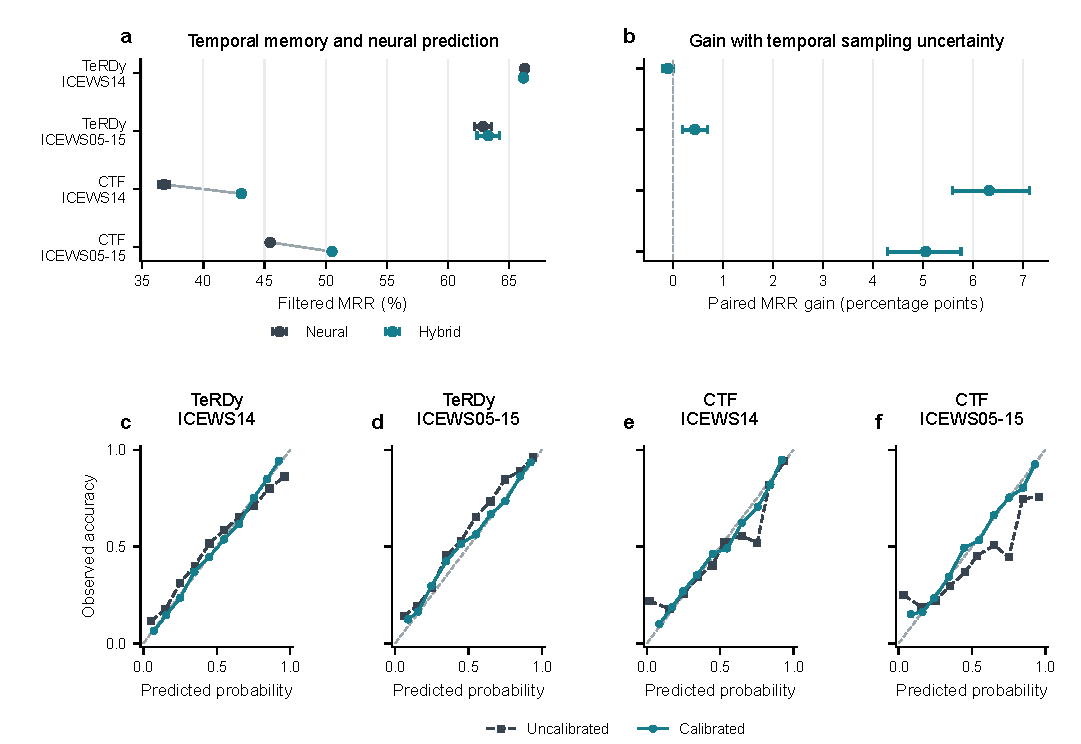
\includegraphics[width=\textwidth]{fig02_prediction.pdf}
\caption{\textbf{Predictive effects and answer calibration across two backbones.}
\textbf{a,} Neural and hybrid MRR on the fixed 5,000-query test panels. Points and bars show three-seed means and sample SD; connecting lines pair the two interfaces.
\textbf{b,} Paired hybrid-minus-neural MRR with 95\% timestamp-block bootstrap intervals from 2,000 draws, conditional on the three fitted models.
\textbf{c--f,} Reliability diagrams for the uncalibrated hybrid maximum and the validation-selected belief model. Each panel pools 15,000 query--seed predictions into ten equal-width probability bins; empty bins are omitted. The dashed diagonal denotes agreement between predicted probability and observed known-answer accuracy. CTF, compact temporal factorization.}
\label{fig:prediction}
\end{figure*}

\subsection{Certified selection exposes an explicit tolerance to deletion}
The exact one-window certificate retained a substantial pool of admissible predictions. Mean certified capacity was 96.75\% and 89.25\% for TeRDy on ICEWS14 and ICEWS05-15, and 59.16\% and 55.14\% for CTF. Some queries had no admissible history: 28.88\% on ICEWS14 and 13.30\% on ICEWS05-15. Restricting the calculation to queries with evidence still gave certified fractions of 95.43\%, 87.60\%, 42.58\% and 48.26\%, respectively. Certification therefore extended beyond the empty-memory fallback.

Applying the certificate as a gate eliminated allowed worst-window flips among accepted answers (Fig.~\ref{fig:selection}; Table~\ref{tab:selection}). Across 60,000 query--seed cases and three deletion budgets, all 180,000 direct witness checks agreed with the certificate, with zero certified violations. At 40\% coverage, the CTF belief selector exposed answers with worst-window flip rates of 32.15\% on ICEWS14 and 10.70\% on ICEWS05-15; the certified policy reduced both rates to zero. Its answer-error rates were 47.78\% and 36.57\%, compared with 46.43\% and 35.28\% for belief alone. The joint rate of an incorrect initial answer or a worst-window flip decreased by 11.07 points (95\% interval 9.36--12.89) and 4.05 points (3.59--4.43). These results quantify the additional stability obtained at the selected coverage and its accompanying correctness trade-off.

Confidence selection already retained almost entirely stable TeRDy answers at low coverage. Its value from the certificate became more visible as coverage increased: at 80\% coverage, joint error decreased by 0.28 points on ICEWS14 and 0.96 points on ICEWS05-15. For the latter interval, 1,748 of 2,000 bootstrap draws retained enough certified queries in every seed, as detailed in the supplement. At the same time, certificate-feature calibration alone had higher mean AURC than the strongest validation-selected control in all four combinations. The gate consequently serves as a defined stability requirement, with confidence and ensemble controls retained as the appropriate comparators for correctness ranking.

\begin{table*}[tbp]\centering\small\caption{Calibrated belief and one-window certified selection on the same predictions. Error and edit-flip rates are percentages at exactly 20\% or 40\% query coverage. Values are three-seed mean $\pm$ SD. Certified capacity is the fraction of all queries passing the certificate. Unavailable coverage is denoted by a dash.}\label{tab:selection}\begin{tabular}{lllrrrr}\toprule Backbone & Dataset & Policy & Error at 20\% & Error at 40\% & Flips at 40\% & Capacity\\\midrule
TeRDy & ICEWS14 & Belief & $8.93\pm3.27$ & $14.70\pm2.70$ & $0.00\pm0.00$ & --\\
TeRDy & ICEWS14 & Certified & $8.93\pm3.27$ & $14.70\pm2.70$ & $0.00\pm0.00$ & $96.75\pm2.08$\\
TeRDy & ICEWS05-15 & Belief & $10.07\pm1.22$ & $18.70\pm0.54$ & $0.03\pm0.06$ & --\\
TeRDy & ICEWS05-15 & Certified & $10.07\pm1.22$ & $18.68\pm0.52$ & $0.00\pm0.00$ & $89.25\pm7.22$\\
CTF & ICEWS14 & Belief & $30.90\pm0.61$ & $46.43\pm0.42$ & $32.15\pm1.66$ & --\\
CTF & ICEWS14 & Certified & $30.97\pm0.81$ & $47.78\pm0.59$ & $0.00\pm0.00$ & $59.16\pm1.64$\\
CTF & ICEWS05-15 & Belief & $21.43\pm0.83$ & $35.28\pm0.51$ & $10.70\pm3.71$ & --\\
CTF & ICEWS05-15 & Certified & $21.43\pm0.83$ & $36.57\pm1.05$ & $0.00\pm0.00$ & $55.14\pm2.18$\\\bottomrule\end{tabular}\end{table*}
\begin{figure*}[tbp]
\centering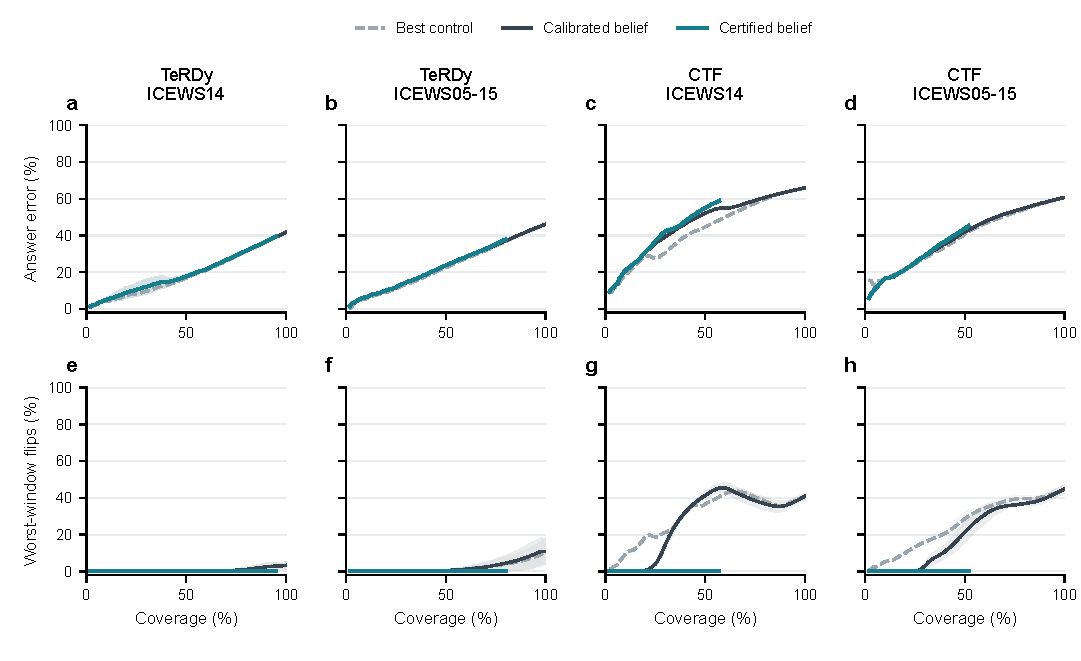
\includegraphics[width=\textwidth]{fig03_selection.pdf}
\caption{\textbf{Correctness and resistance to evidence deletion are separate selection objectives.}
\textbf{a--d,} Answer-error risk--coverage curves for the best validation-selected control, the one-encoder calibrated belief policy and its one-window certified gate.
\textbf{e--h,} The corresponding worst-case one-window flip rates, evaluated on exactly the same selected predictions. Curves show three-seed means; bands show sample SD. A certified curve stops at the largest plotted coverage reachable by every seed. Controls include temperature scaling and a three-seed ensemble, and their identities are frozen on validation data. Each panel uses all 5,000 test queries per seed.}
\label{fig:selection}
\end{figure*}

\subsection{Certificate surplus predicts vulnerability beyond the original partition}
The surplus retained diagnostic value when the intervention changed (Fig.~\ref{fig:diagnostics}). For random two-window deletions, shifted window boundaries, doubled window width and single-event deletion, its AUROC exceeded that of the original hybrid margin in every backbone--dataset combination. The 16 paired gains ranged from 0.064 to 0.584, and every 95\% interval lay above zero. On TeRDy, where margin was already informative, the surplus reached AUROCs of 0.991--0.998 on ICEWS14 and 0.970--0.992 on ICEWS05-15. For CTF, the corresponding ranges were 0.903--0.969 and 0.847--0.982.

This diagnostic comparison concerns direct interventions on the same fixed predictions. A large current score gap can arise from highly concentrated memory support, whereas the surplus accounts for how that gap changes when shared evidence is removed. The conceptual equal-score example in Fig.~\ref{fig:interface} isolates this distinction exactly, and the public-data perturbations show its empirical relevance across different evidence partitions. The formal guarantee remains tied to the declared window family; the alternative interventions measure how informative the score remains outside that exact family.

\begin{figure*}[tbp]
\centering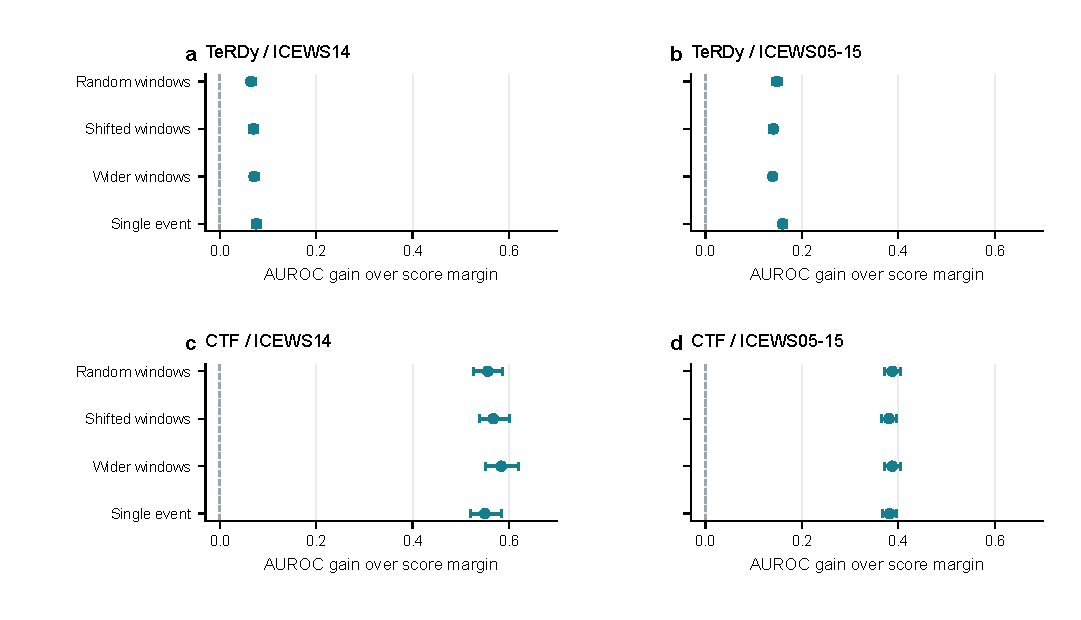
\includegraphics[width=\textwidth]{fig04_diagnostics.pdf}
\caption{\textbf{The certificate surplus identifies edit-sensitive answers more accurately than the original score margin.}
\textbf{a--d,} AUROC differences between negative one-window surplus and negative hybrid margin for the four indicated backbone--dataset combinations. The outcomes are an answer change under at least one of eight random two-window deletions, a worst-case shifted seven-unit window deletion, a worst-case 14-unit window deletion, and removal of the latest winner-supporting event. Each comparison pools 15,000 query--seed predictions. Bars show paired 95\% intervals from 2,000 timestamp-block bootstrap draws, resampled jointly across the three fixed fits.}
\label{fig:diagnostics}
\end{figure*}

\subsection{Exact certification resolves the cost of conservative and sampled checks}
Exact certification recovered admissible answers that a conservative bound rejected (Fig.~\ref{fig:controls}a). Among queries with nonempty memory, its one-window certified coverage exceeded the winner-only bound by 2.45 and 12.09 percentage points for TeRDy on ICEWS14 and ICEWS05-15, and by 2.28 and 2.49 points for CTF. The largest difference arose on TeRDy/ICEWS05-15, where coverage increased from 80.39\% to 92.48\%. Accounting for the competitor's simultaneous evidence loss therefore makes the guarantee more useful without relaxing the deletion budget.

Finite deletion probes had a different limitation (Fig.~\ref{fig:controls}b). On CTF/ICEWS05-15, 31.93\% of nonempty-memory queries that passed eight probes were vulnerable to another allowed deletion. Increasing the probe count to 32 and 64 reduced this fraction to 18.60\% and 11.35\%, respectively. At 64 probes, the corresponding fractions were 0\%, 0.67\% and 1.57\% for TeRDy/ICEWS14, TeRDy/ICEWS05-15 and CTF/ICEWS14. The exact certificate resolves this residual uncertainty by covering every allowed subset analytically.

The prespecified weight sweep explains why the predictive operating point is selected separately from the deletion budget (Fig.~\ref{fig:controls}c,d). Greater memory weight increased CTF MRR over its neural-only value throughout the grid, while the strongest TeRDy performance occurred at smaller weights. Certified capacity decreased as memory acquired more influence in these measurements. The complete sweep, including $\lambda=0$, is reported in the supplement. A fixed-denominator calculation disagreed with the renormalized one-window certificate on 0.14--8.22\% of all queries, demonstrating that the edited-score definition also matters.

Sparse competitor reduction made the exact calculation practical. Over the 32-query microbenchmark, including empty-memory queries, median paired dense-to-sparse runtime ratios were 4.63--11.75 across the four combinations. On nonempty histories they were 7.50--17.52. These timings compare a sparse implementation returning certificates, radius and witnesses with a dense implementation returning certificate indicators; all-query and nonempty-history timings are reported separately in the supplement. Together, the controls distinguish exact certification from both conservative abstention and finite intervention sampling.

\begin{figure*}[tbp]
\centering
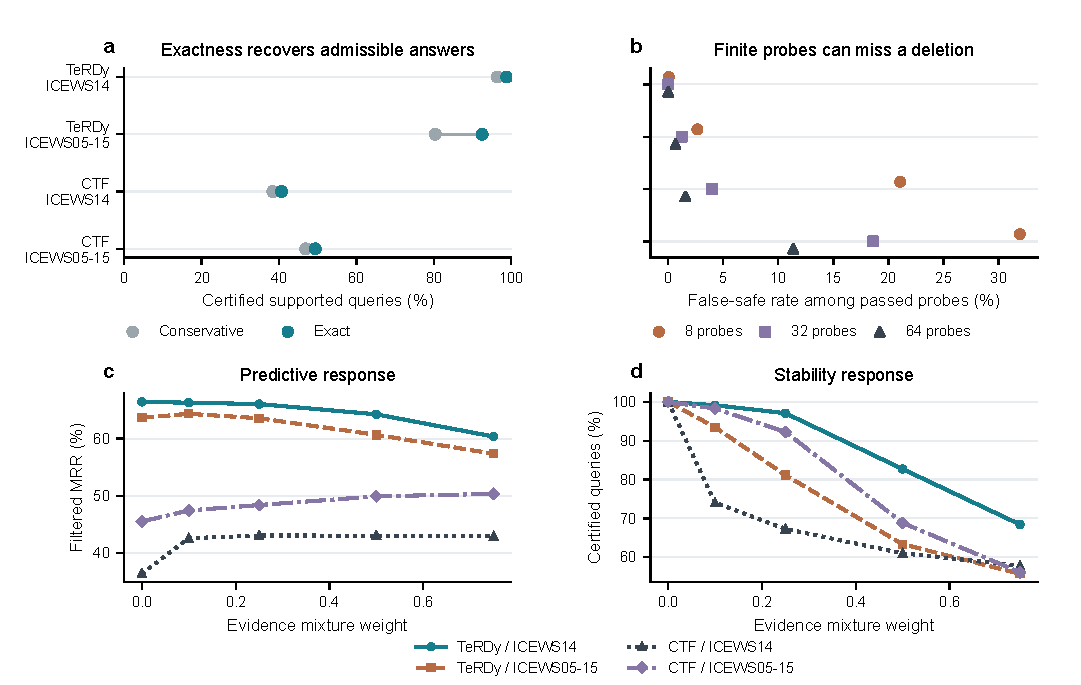
\includegraphics[width=\textwidth]{fig05_controls.pdf}
\caption{\textbf{Analytical exactness and the evidence-weight trade-off.}
\textbf{a,} Exact and conservative one-window certificate coverage among queries with nonempty memory.
\textbf{b,} The fraction of predictions passing all sampled deletion probes that are vulnerable to the exact one-window adversary, for 8, 32 and 64 probes.
\textbf{c,d,} Filtered MRR and one-window certified coverage over the prespecified evidence-weight grid. These controls use seed 0 of every backbone--dataset combination and all 5,000 test queries; temperature is held at its validation-selected value.}
\label{fig:controls}
\end{figure*}

\subsection{Local maintenance restricts recomputation to affected answers}
Local maintenance reduced the number of refreshed query states from 1,200,000 to 55,064 across all 240 transactions, a reduction of 95.41\% (Fig.~\ref{fig:maintenance}). The reductions were 95.59\%, 94.21\% and 96.44\% on ICEWS14, ICEWS05-15 and GDELT, respectively. Both implementations applied identical event writes and maintained identical window statistics; the difference was whether every registered query or only the affected set was refreshed. Their outputs agreed after every transaction, and independent raw-event rebuilds agreed on all discrete outputs for 128 queries per dataset, with maximum absolute numerical difference $2.22\times10^{-16}$.

The benefit remained measurable at the largest transaction size. For 1,000 edited events, median local refresh times were 0.330, 2.407 and 0.504 seconds on the three datasets, compared with 1.367, 4.030 and 2.161 seconds for full refresh. The median paired speedups were 4.18, 1.67 and 4.29, respectively. Median affected sets contained 739, 973.5 and 631.5 of the 5,000 registered queries. Smaller transactions touched fewer answers and produced larger timing ratios. Uniformly sampled single-event edits affected no registered query in 80\%, 60\% and 20\% of transactions, respectively; the supplement reports these frequencies alongside every timing stratum.

Initial cache construction took 2.20--5.46 seconds. Numeric arrays occupied 283, 700 and 275~MiB on ICEWS14, ICEWS05-15 and GDELT; measured process-memory increments, including container overhead, were 434, 951 and 305~MiB. These one-time costs are separated from transaction timings. The results show that explicit evidence dependencies support both the stability calculation and its efficient maintenance, including on the larger GDELT event history.

\begin{figure*}[tbp]
\centering
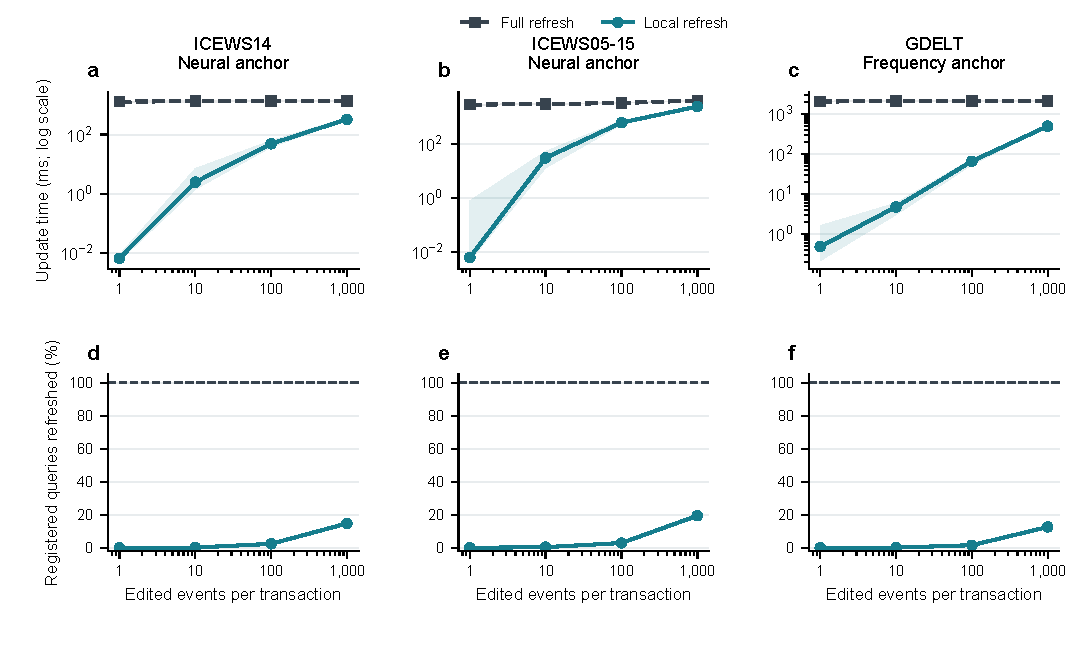
\includegraphics[width=\textwidth]{fig06_maintenance.pdf}
\caption{\textbf{Maintaining only affected answers reduces update work.}
\textbf{a--c,} Full and local refresh times for 5,000 registered queries after transactions of 1, 10, 100 or 1,000 events. Points show medians and bands show interquartile ranges over ten sampled deletion/restoration pairs at each batch size, with alternating implementation order.
\textbf{d--f,} The corresponding fraction of registered queries refreshed. The full control refreshes 100\% at every transaction. Timings include event writes and certificate maintenance; encoder inference and initial cache construction are excluded. GDELT uses a fixed training relation-frequency anchor and tests maintenance scaling.}
\label{fig:maintenance}
\end{figure*}


\section{Discussion}
\StableKG{} turns an answer's response to evidence withdrawal into an explicit inference property. The certificate captures how support is organized across temporal windows, a property that the unedited score vector alone cannot identify (Fig.~\ref{fig:interface}). Connecting this property to calibrated selection and locally maintained memory gives a common interface for prediction, acceptance and revision. The same evidence representation supports both the guarantee used to accept an answer and the computation used to revisit it.

The distinction between confidence and edit stability is central to interpreting the evidence. Confidence controls already rank correctness effectively for the stronger backbone. A certificate supplies a different capability: it identifies predictions whose answer is invariant to every allowed window deletion. The perturbation results show that the signed surplus also contains useful information about vulnerability beyond the original partition. Consequently, certification can be used as an explicit acceptance requirement even when its features add little to a correctness calibrator. This separation makes the system's decision interpretable: the probability concerns empirical correctness, and the certificate concerns a specified intervention.

This contribution complements recent temporal conformal prediction and interpretable graph editing. NCPNET addresses prediction-set coverage under non-exchangeable temporal observations \citep{wang2025nonexchangeable}; IGETR uses graph paths and language-model-guided editing to improve reasoning \citep{fan2026editing}. The present guarantee is a deterministic property of one fixed answer under memory withdrawal. Its exactness comes from a structured inference interface, whereas sampled robustness methods such as GraphProt and AdaptDel obtain guarantees through their own randomized constructions and perturbation models \citep{yang2025graphprot,huang2025adaptdel}. These differences suggest a modular division of labor: expressive encoders represent temporal knowledge, statistical selectors estimate answer reliability, and explicit evidence channels make selected revisions exactly analyzable.

The mixture also exposes a useful design choice. Increasing the contribution of temporal memory changes both predictive performance and sensitivity to that memory. The strong and compact backbones occupy different parts of this trade-off, so a common accuracy benefit is not required for a common certificate interface. Validation chooses the predictive operating point, while a deletion budget specifies the tolerated intervention. The guarantee applies to the frozen encoder, fixed admissible vocabulary and declared window family. Extending it to encoder retraining, arbitrary counter-evidence insertion or a continually changing candidate set requires additional analysis. Chronological forecasting and application-defined withdrawal windows are natural next tests of the interface.

Local maintenance makes this interpretation operational. The reverse index identifies exactly which registered queries depend on an edited event, and the measured comparison includes the writes and certificate refresh on both paths. The result is a system in which prediction, acceptance and revision share an explicit evidence representation. This provides a concrete basis for exposing neural knowledge-graph answers together with an inspectable tolerance to change.

\section{Conclusion}
\StableKG{} equips neural temporal knowledge graph completion with exact shared-window deletion certificates, calibrated certified selection and local evidence maintenance. The ratio-to-additive reduction and sparse competitor theorem make this capability computationally accessible, while public-data experiments establish its predictive, diagnostic and maintenance behavior. Together, these results provide a reproducible route to neural answers whose response to evidence withdrawal can be specified, certified and efficiently maintained.

\FloatBarrier
\section*{CRediT authorship contribution statement}
Yanbo Bian: Conceptualization, Methodology, Software, Validation, Formal analysis, Investigation, Data curation, Visualization, Writing -- original draft, Writing -- review and editing.
\section*{Funding}
This research received no external funding.
\section*{Declaration of competing interest}
The author declares no known competing financial interests or personal relationships that could have appeared to influence the work reported in this paper.
\section*{Data availability}
The ICEWS14, ICEWS05-15 and GDELT query-format distributions are publicly available from the TFLEX dataset mirrors. Immutable archive URLs, source terms and SHA-256 hashes are provided in the repository data manifest. Query-level results and figure source data accompany the Neurocomputing release at \url{https://github.com/bianyanbo44-afk/stablekg-kbs/tree/neurocomputing-v1}.
\section*{Code availability}
The implementation, fixed configurations, data preparation, experiment entry points, tests, figure scripts and editable manuscript sources are available at \url{https://github.com/bianyanbo44-afk/stablekg-kbs/tree/neurocomputing-v1}. External model implementations are referenced at their original pinned revisions and retain their source terms.
\section*{Declaration of generative AI and AI-assisted technologies in the preparation process}
OpenAI Codex was used to assist software development, experiment execution, data analysis, figure preparation and manuscript drafting. Numerical findings were generated by the accompanying executable analyses. The author takes responsibility for the submitted content.
\bibliographystyle{elsarticle-num}
\balance
\bibliography{references}
\end{document}
